В настоящем параграфе будут даны инструкции для разворачивания инфраструктуры сборки проекта
для операционных систем Linux(Ubuntu), MacOS и Windows.

В процессе настройки будет необходимо установить систему контроля версий {\bf Git},
систему контейнеризации {\bf Docker} и (опционально) интегрированную среду разработки.
Проект позволяет работать в любой среде разработки.
Ниже будут приведены инструкции для настройки {\bf vscode}.

Процесс сборки и запуска программ будет осуществляться в системе, развёрнутой в докере на основе Ubuntu 24.04.
В дальнейшем систему, установленную непосредственно на компьютере, будем называть хост системой.
А систему, развёрнутую в докере -- контейнером.

Для успешной установке на хосте должно быть около 5Гб свободного места.

\subsection{Клонирование}
Для клонирования проекта на локальный компьютер необходимо установить систему контроля версий Git
и открыть терминал на хост-системе в папке, в которой планируется хранить папку с репозиторием.
Если в качестве это папки будет использоваться домашняя пользовательская папка.
В нижеследующих инструкциях в качестве такой папки будет использоваться домашняя папка пользователя.

\begin{center}

\begin{tcolorbox}[osstyle, title=Ubuntu]
Откройте терминал и в нём
\begin{shelloutput}
sudo apt install git  # установка гита
cd ~                  # переходим в папку,
                      # где будет хранится папка с репозиторием
\end{shelloutput}
\end{tcolorbox}

\begin{tcolorbox}[osstyle, title=Windows]
В Windows необходимо скачать и установить дистрибутив
\url{https://github.com/git-for-windows/git/releases/download/v2.51.0.windows.1/Git-2.51.0-64-bit.exe}.
Далее откройте командную строку \ename{cmd}. И в ней перейдите в целевую папку
\begin{shelloutput}
cd %USERPROFILE%
\end{shelloutput}
\end{tcolorbox}

\begin{tcolorbox}[osstyle, title=MacOs]
Откройте терминал и в нём
\begin{shelloutput}
# Установите Homebrew, если у вас его ещё нет
/bin/bash -c \
"$(curl -fsSL https://raw.githubusercontent.com/Homebrew/install/HEAD/install.sh)"
# установка гита
brew install git
# переходим в папку где будет хранится папка с репозиторием
cd ~                  
\end{shelloutput}
\end{tcolorbox}

\end{center}

Далее необходимо клонировать репозиторий

\begin{shelloutput}
git clone https://github.com/kalininei/CFDCourse26
\end{shelloutput}

В результате в домашней папке должна появиться папка с \ename{CFDCourse26}.

\subsection{Разворачивание контейнера}

Установим докер

\begin{tcolorbox}[osstyle, title=Ubuntu+apt]
Запустить скрипт, написанный на основе инструкций с официального сайта \url{https://docs.docker.com/engine/install/ubuntu/#install-using-the-repository}:
\begin{shelloutput}
cd ~/CFDCourse26    # перейдём в репозиторий
./scripts/ubuntu_docker_install.sh
\end{shelloutput}
\end{tcolorbox}

\begin{tcolorbox}[osstyle, title=Windows/MacOs+DockerDesktop]
Скачайте и установите дистрибутив с официального сайта 
\begin{itemize}
\item \url{https://docs.docker.com/desktop/setup/install/windows-install/} для Windows
\item \url{https://docs.docker.com/desktop/setup/install/mac-install/} для MacOs
\end{itemize}
Далее следуйте процедуре установки десктопного приложения.
После установки запустите \ename{DockerDesktop}.
Этап регистрации при запуске опционален и может быть пропущен.
\end{tcolorbox}

Далее в терминале находясь в директории \ename{CFDCourse26} развернём контейнер:
\begin{shelloutput}
docker compose up --build -d
\end{shelloutput}
На этом этапе будет скачаны необходимые образы и запущен контейнер.
По окончании можно убедится, что контейнер работает
\begin{shelloutput}
docker ps
\end{shelloutput}
В случае работы с \ename{DockerDesctop} запущенный контейнер будет виден в графическом интерфейсе во вкладке \ename{Containers}.

\subsection{Базовая разработка}
\label{sec:howto_basic_dev}
Чтобы скомпилировать проект необходимо войти в терминал контейнера.
Далее
\begin{shelloutput}
docker ps                   # Убедимся, что контейнер cfd26 запущен
docker exec -it cfd26 bash  # Войдём в него
\end{shelloutput}
Папка хоста с репозиторием \ename{CFDCourse} примонтирована к папке контейнера \ename{/app}.
Войдём туда
\begin{shelloutput}
cd /app   # заходим в директорию
ls -alh   # смотрим список файлов
\end{shelloutput}
Для удобства в контейнере установлен консольный файловый менеджер \ename{mc},
который можно использовать для операций с файлами. Так же есть его псевдоним \ename{mcc},
который отличается от базового \ename{mc} тем, что запоминает текущую директорию при выходе.
Благодаря чему его можно использовать для навигации вместо \ename{cd}.

\subsubsection{Особенности проекта}
\begin{itemize}
\item Проект состоит из статически линкуемой библиотеки \ename{libcfd26.a} и исполняемого файла \ename{cfd26_test} с тестовыми программами для этой библиотеки.
      Исходники библиотеки лежат в директории \ename{src/cfd}, исходники тестов -- \ename{src/test},
\item Используется 20-ый стандарт C++,
\item Сборка осуществляется в системе cmake,
\item Для написания тестов используется фреймворк \ename{Catch2},
\item В проекте установлены жёсткие правила работы с предупреждениями компилляции, из-за которых они как обрабатываются ошибки,
\item В проекте установлены форматтеры для исходных кодов на С++, python, cmake. При сохранении любого исходного файла этих форматов в vscode
      форматтер будет вызван автоматически. Если исходники модифицировались иначе, то запустить форматтер для всех файлов проекта
      можно скриптом \ename{scripts/formatall.sh} из папки \ename{/app}.
\end{itemize}

\subsubsection{Сборка в отладочном режиме}
Из папки \ename{/app} контейнера:
\begin{shelloutput}
mkdir build                        # создаём папку, в которую будут строится программа
cd build                           # Заходим
cmake .. -DCMAKE_BUILD_TYPE=Debug  # Строим сборочные скрипты
make -j4                           # Компилируем на 4-х потоках
\end{shelloutput}
Сама папка \ename{build} является временной папкой для построения.
Она не подключена к системе контроля версий.  И может быть удалена и создана заново (например для полной гарантированной очистки кэша построения).
Бинарные файлы будут построены в папку \ename{/app/build/bin}.
Для запуска тестов зайдём в эту папку:
\begin{shelloutput}
cd bin
./cfd26_test                # запуск всех тестов
./cfd26_test [grid1]        # запуск единственного тест кейса
\end{shelloutput}

\subsubsection{Сборка в релизном режиме}
Отличается от сборки в отладочном режиме только флагом \ename{cmake}.
Будем строить в папку \ename{build_release}.
Также от папки \ename{/app}
\begin{shelloutput}
mkdir build_release                         # создаём папку
cd build_release                            # Заходим
cmake .. -DCMAKE_BUILD_TYPE=RelWithDebInfo  # Или просто Release,
                                            # если отладочная информация не нужна
make -j4                                    # Компилируем на 4-х потоках
cd bin                                      # заходим в папку с исполняемым файлом
./cfd26_test                                # запуск всех тестов
./cfd26_test [grid1]                        # запуск единственного тест кейса
\end{shelloutput}

\subsubsection{Работа с кодом}
Работать с исходными файлами можно находясь на хосте и используя любой удобный текстовый редактор.
(например \ename{notepad++} на Windows).
Порядок работы будет выглядеть следующим образом
\begin{itemize}
\item Редактировать исходные файлы на хосте в папке \ename{CFDCourse26/src}
\item Для сборки переключиться на терминал и выполнить вышеописанную процедуру сборки
\item Если сборка не прошла из-за ошибок в коде, эти ошибки будут распечатаны в терминал с указанием файла и номера строки
\item Для отладки можно использовать консольный отладчик \ename{gdb} из терминала
\end{itemize}

\subsection{Разработка в vscode}
\subsubsection{Подключение к контейнеру}
Необходимо установить vscode на хосте следуя инструкциям с официального сайта \url{https://code.visualstudio.com/Download}.
В самом vscode нужно установить расширение \ename{Remote Explorer, Dev Containers} для удалённой разработки в контейнере. 
Далее нужно переключиться на вкладку RemoteExplorer (см. рис.~\ref{fig:vscode_to_docker}).

\begin{figure}[h]
\centering
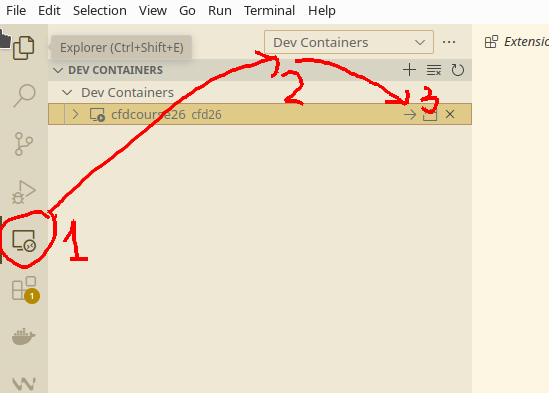
\includegraphics[width=0.6\linewidth]{attach_vscode_to_docker.png}
\caption{Подключения vscode к контейнеру}
\label{fig:vscode_to_docker}
\end{figure}

\subsubsection{Настройки vscode}
Далее необходимо открыть папку \ename{/app}: \ename{File->Open Folder...}.
Контейнер содержит в себе базовые настройки vscode, которые при сборке контейнера
копируются в папки \ename{.vscode, .vscode-server}.

Следует отметить, что удалённо подключённый vscode не может пользоваться
расширениями, установленными на хосте. Все необходимые расширения нужно устанавливать в контейнер заново.
Список базовых расширений, необходимых для работы, уже содержится в настроечных файлах.
Когда вы откроете папку \ename{app} в vscode, вам будет предложено эти расширения установить. Нужно согласиться.

Настроечные папки \ename{.vscode, .vscode-server} игнорируются системой контроля версий и расположены на хосте.
То есть вы можете дополнительно установить туда любые свои расширения и донастроить vscode как вам удобно.
Эти настройки не будут зависеть от ветки гита и не будут затираться при пересборке контейнера.

Если всё же понадобится обнулить настройки vscode, нужно
\begin{enumerate}
\item удалить папки \ename{.vscode, .vscode_server}
\item удалить все настройки из конфигурационного файла контейнера (\ename{ctrl+shift+p, open container configuration file})
\item выйти из контейнера на vscode: \ename{File->Close Remote Connection}
\item остановить и пересобрать контейнер на хосте
\begin{shelloutput}
docker stop cfd26
docker compose up --build -d
\end{shelloutput}
\end{enumerate}

\subsubsection{Сборка и отладка}
В папке \ename{.vscode} лежат базовые таски и лаунчи для компилляции и запуска программы.
В случае необходимости можете дополнить базовый набор своими командами.
Согласно настройкам по умолчанию
по нажатию \ename{F5} происходит сборка программы в отладочном режиме и запуск отладки
тестовой программы с прогоном всех тестов.
Посмотреть результаты можно на вкладке \ename{TERMINAL}.
В случае ошибок компилляции, список этих ошибок будет виден на вкладке \ename{PROBLEMS}.

Для отладки конкретного теста необходимо запустить тестовую программу с аргументом (например \cvar{cfd26_test [grid1]}.
Чтобы передать программе аргумент нужно этот аргумент прописать в файле \ename{.vscode/launch.json}
в поле \ename{args}. Либо создать ещё одну конфигурацию запуска с вашими аргументами и указать эту конфигурацию в настройке \ename{Run And Dubug}.

Чтобы собрать программу без запуска нужно выполнить таск (\ename{ctrl+shift+b}): \ename{cmake: build debug, cmake: build release}
для отладочного и релизного режима соответственно. 

В целом сборка на vscode представляет из себя автоматизированный алгоритм, представленный в п.~\ref{sec:howto_basic_dev}.
То есть исполняемая программа в дебаговой версии кладётся в папку \ename{build}, в релизной -- в \ename{build_release} и её можно запустить из терминала.
Удаление этих папок ведёт к полной очистке кэша построения.

